\chapter{Haar Measure, the Weyl Criterion and Sato Tate}\label{ch:04}

In 1916 Hermann Weyl showed that a sequence in $[0,1)$ is equidistributed if and only if the averages of the characters $e^{2\pi i h x}$ along it tend to zero for every integer $h \neq 0$ \cite{weyl1916}. He used the criterion to reprove the equidistribution of the fractional parts of $n\alpha$ for irrational $\alpha$, found around 1910 by Bohl, Sierpi\'nski and Weyl himself, and to extend it to polynomial sequences; the criterion has outlived the problem. The Peter Weyl theorem \cite{peterweyl1927}, proved in 1927 for compact Lie groups, makes the matrix coefficients of irreducible representations dense among continuous functions and so gives the same criterion on compact groups, with irreducible characters in place of exponentials. In the early 1960s Sato and Tate, working independently and from quite different directions, predicted that the angles of Frobenius of an elliptic curve over $\Q$ without complex multiplication are distributed according to the image of Haar measure on $\SU(2)$ \cite{tate1965}. Serre saw that Weyl's criterion converts this prediction into a statement about $L$ functions \cite{serre1968}: the conjecture follows if every symmetric power $L$ function is holomorphic and nonvanishing on the line $\Re s = 1$. That statement is a consequence of functoriality. For elliptic curves over $\Q$ and holomorphic newforms it was proved through potential automorphy in papers published between 2008 and 2011, and in 2021 Newton and Thorne proved that every symmetric power is automorphic; this is one of the clearest successes of the Langlands programme. We prove the probabilistic side completely and state the arithmetic input precisely. The logical direction matters throughout: automorphy is the input, equidistribution is the output.

\section{Equidistribution on compact metric spaces}

Let $X$ be a compact metric space and $\mu$ a Borel probability measure on $X$. A sequence $(x_j)$ in $X$ is \emph{equidistributed} with respect to $\mu$ if the empirical measures $\nu_n = n^{-1}\sum_{j\le n}\delta_{x_j}$ converge weakly to $\mu$, that is $\int f\,d\nu_n \to \int f\,d\mu$ for every $f \in C(X)$.\index{equidistribution} For sequences indexed by primes we use the ordering by size, so the natural normalisation is $\pi(x)^{-1}\sum_{p\le x}$.

Weak convergence can be tested on any family of functions whose linear span is dense in $C(X)$ for the supremum norm. This observation is the whole content of the Weyl criterion; what makes it useful is that representation theory supplies a canonical dense family. For the circle $\R/\Z$ the family is $x \mapsto e^{2\pi ihx}$, $h \in \Z$, whose span is dense by Fej\'er's theorem; this recovers Weyl's original criterion. We shall also use the portmanteau theorem: if $\nu_n \to \mu$ weakly, then $\limsup \nu_n(F) \le \mu(F)$ for every closed $F \subset X$.

\section{Peter Weyl and Schur orthogonality}

Let $K$ be a compact metrisable group, for instance a closed subgroup of $\mathrm{U}(n)$, with normalised Haar measure $h$. Representations of $K$ are continuous and finite dimensional. A \emph{class function} is a function constant on conjugacy classes. Write $K^\natural$ for the space of conjugacy classes with the quotient topology, a compact metrisable space, and $h^\natural$ for the pushforward of $h$. Continuous class functions on $K$ are exactly the continuous functions on $K^\natural$. For a representation $\rho$ of $K$ we write $\chi_\rho = \tr \rho$ for its character.

\begin{theorem}[Schur orthogonality]\index{Schur orthogonality}
If $\rho$ and $\sigma$ are irreducible representations of $K$, then
\[
\int_K \chi_\rho(g)\overline{\chi_\sigma(g)}\,dh(g) =
\begin{cases} 1 & \rho \cong \sigma,\\ 0 & \text{otherwise.}\end{cases}
\]
In particular $\int \chi_\rho\,dh = 0$ for every nontrivial irreducible $\rho$.
\end{theorem}

\begin{theorem}[Peter and Weyl \cite{peterweyl1927}]\index{Peter Weyl theorem}
Matrix coefficients of finite dimensional irreducible representations span a dense subspace of $C(K)$. Consequently the characters of irreducible representations span a dense subspace of the continuous class functions on $K$.
\end{theorem}

The second statement follows from the first. The averaging operator $P\phi(g) = \int_K \phi(kgk^{-1})\,dh(k)$ fixes class functions, does not increase the supremum norm, and, by Schur's lemma, maps each matrix coefficient of an irreducible $\rho$ to a multiple of $\chi_\rho$. So if a class function $f$ satisfies $\|f - \phi\|_\infty < \delta$ for a combination $\phi$ of matrix coefficients, then $\|f - P\phi\|_\infty < \delta$, and $P\phi$ is a combination of irreducible characters.

\section{The Weyl criterion on compact groups}

We prove the form of the criterion used throughout the book.

\begin{theorem}[Weyl criterion \cite{weyl1916,serre1968}]\label{thm:04weyl}\index{Weyl criterion}
Let $K$ be a compact metrisable group and $(\theta_p)$ a sequence in $K^\natural$ indexed by primes. Then $(\theta_p)$ is equidistributed with respect to $h^\natural$ if and only if, for every nontrivial irreducible representation $\rho$ of $K$,
\[
\lim_{x\to\infty}\frac{1}{\pi(x)}\sum_{p\le x}\chi_\rho(\theta_p) = 0 .
\]
More generally, $(\theta_p)$ is equidistributed with respect to a probability measure $\mu$ on $K^\natural$ if and only if $\pi(x)^{-1}\sum_{p\le x}\chi_\rho(\theta_p) \to \int \chi_\rho\,d\mu$ for every irreducible $\rho$.
\end{theorem}

\begin{proof}
We prove the general statement; the first follows from Schur orthogonality, which gives $\int \chi_\rho\,dh^\natural = 0$ for nontrivial $\rho$ and $1$ for the trivial representation. Write $\nu_x = \pi(x)^{-1}\sum_{p\le x}\delta_{\theta_p}$.

Necessity is immediate: each $\chi_\rho$ is continuous on $K^\natural$.

For sufficiency, let $f \in C(K^\natural)$ and $\delta > 0$. By the Peter Weyl theorem there is a finite linear combination $g = \sum_\rho c_\rho\chi_\rho$ with $\|f - g\|_\infty < \delta$. By hypothesis and linearity, $\int g\,d\nu_x \to \int g\,d\mu$. Then
\[
\Bigl|\int f\,d\nu_x - \int f\,d\mu\Bigr|
\le \Bigl|\int (f-g)\,d\nu_x\Bigr| + \Bigl|\int g\,d\nu_x - \int g\,d\mu\Bigr| + \Bigl|\int (g-f)\,d\mu\Bigr| ,
\]
and the first and third terms are each at most $\delta$ because $\nu_x$ and $\mu$ are probability measures. Hence $\limsup_x |\int f\,d\nu_x - \int f\,d\mu| \le 2\delta$ for every $\delta > 0$, and the limit is $0$.
\end{proof}

The proof uses only that each $\nu_x$ is a probability measure on $K^\natural$. The criterion therefore holds for any sequence of probability measures on $K^\natural$, for instance the empirical measures $n^{-1}\sum_{j\le n}\delta_{\theta_j}$ of a sequence indexed by the integers, or those of the finite families of conjugacy classes that arise in vertical problems (Chapter~\ref{ch:06b}).

The limits $\int \chi_\rho\,d\mu$ for a measure other than Haar are themselves informative: when $\mu$ is the image of Haar measure on a closed subgroup $H \subset K$, the integral is the multiplicity of the trivial representation in $\rho|_H$, a nonnegative integer. We call the function $\rho \mapsto \int \chi_\rho\,d\mu$ on the irreducible representations of $K$ the \emph{Weyl fingerprint}\index{Weyl fingerprint} of $\mu$; for $\SU(2)$ it is a sequence indexed by $n \ge 0$ (next section).

\section{The group SU(2)}

Every element of $\SU(2)$ is conjugate to $\operatorname{diag}(e^{i\theta}, e^{-i\theta})$ for a unique $\theta \in [0,\pi]$, so $\SU(2)^\natural$ is identified with $[0,\pi]$, and equally with the interval $[-2,2]$ through the trace $x = 2\cos\theta$. The irreducible representations are the symmetric powers $\Sym^n$ of the standard representation, of dimension $n+1$, with eigenvalues $e^{i(n-2j)\theta}$ for $0\le j\le n$. Summing the geometric progression,
\[
\chi_n(\theta) = \tr\Sym^n(\theta) = \sum_{j=0}^n e^{i(n-2j)\theta} = \frac{\sin((n+1)\theta)}{\sin\theta} = U_n(\cos\theta) = U_n(x/2),
\]
where $U_n$ is the Chebyshev polynomial of the second kind.\index{Chebyshev polynomials} The recurrence $U_1(t)U_n(t) = U_{n+1}(t) + U_{n-1}(t)$ is the Clebsch Gordan rule $\mathrm{std}\otimes\Sym^n \cong \Sym^{n+1}\oplus\Sym^{n-1}$.

\begin{proposition}[Weyl integration formula for $\SU(2)$]\index{Weyl integration formula}
The pushforward of Haar measure to $[0,\pi]$ is $\frac{2}{\pi}\sin^2\theta\,d\theta$. Equivalently, the trace $x = 2\cos\theta$ of a Haar random element has the semicircle law
\[
\ST(dx) = \frac{1}{2\pi}\sqrt{4 - x^2}\,dx, \qquad x \in [-2,2].
\]
\end{proposition}

\begin{proof}
Identify $\SU(2)$ with the unit quaternions $S^3$; Haar measure is normalised surface measure, since multiplications by unit quaternions are isometries. The trace is $2a$ for $g = a + bi + cj + dk$, and the slice $\{a = \cos\theta\}$ is a two sphere of radius $\sin\theta$, so surface measure on $S^3$ projects to a density proportional to $\sin^2\theta$ on $[0,\pi]$. Since $\int_0^\pi \sin^2\theta\,d\theta = \pi/2$, the normalised density is $\frac{2}{\pi}\sin^2\theta$. Changing variables $x = 2\cos\theta$, $dx = -2\sin\theta\,d\theta$ and $\sin\theta = \frac12\sqrt{4-x^2}$ gives the semicircle.
\end{proof}

\begin{proposition}[Orthonormality and Catalan moments]\label{prop:04catalan}
The polynomials $U_n(x/2)$ are orthonormal in $L^2(\ST)$, and
\[
\int_{-2}^2 x^{k}\,\ST(dx) = \begin{cases} C_m = \dfrac{1}{m+1}\dbinom{2m}{m} & k = 2m,\\[4pt] 0 & k \text{ odd.}\end{cases}
\]
\end{proposition}

\begin{proof}
In the variable $\theta$, the factors $\sin\theta$ cancel against the density $\frac{2}{\pi}\sin^2\theta$, and
\[
\int U_m(x/2)\,U_n(x/2)\,\ST(dx) = \frac{2}{\pi}\int_0^\pi \sin((m+1)\theta)\sin((n+1)\theta)\,d\theta = \delta_{mn}
\]
by orthogonality of sines on $[0,\pi]$.

For the moments, iterate the Clebsch Gordan rule. Since $x = U_1(x/2)$, we have $x\,U_n(x/2) = U_{n+1}(x/2) + U_{n-1}(x/2)$ for $n \ge 1$ and $x\,U_0(x/2) = U_1(x/2)$. By induction $x^k = \sum_{n\ge0} N_k(n)\,U_n(x/2)$, where $N_k(n)$ is the number of paths of $k$ steps $\pm1$ on the nonnegative integers from $0$ to $n$ that never go below $0$. By orthonormality, $\int x^k\,d\ST = N_k(0)$, the number of Dyck paths of length $k$. This vanishes for $k$ odd, and for $k = 2m$ the reflection principle gives $N_{2m}(0) = \binom{2m}{m} - \binom{2m}{m+1} = C_m$.
\end{proof}

The moments of $\ST$ thus count returning paths of the simple walk on the nonnegative integers. Spectral measures whose moments count returning paths recur throughout the book; in Chapter~\ref{ch:07} the same computation on a regular tree produces the Kesten McKay laws.

\section{The Sato Tate conjecture and Serre's theorem}

Let $E/\Q$ be an elliptic curve of conductor $N$. For $p \nmid N$ put $a_p = p + 1 - \#E(\mathbb{F}_p)$. Hasse's bound $|a_p| \le 2\sqrt p$ says that $x_p = a_p/\sqrt p$ lies in $[-2,2]$, so we may write $x_p = 2\cos\theta_p$ with $\theta_p \in [0,\pi]$, and regard $\theta_p$ as the conjugacy class in $\SU(2)$ of the normalised Frobenius. More generally, for a holomorphic newform $f = \sum a_n q^n$ of weight $k \ge 2$, level $N$ and trivial character, Deligne's theorem \cite{deligne1974} gives $|a_p| \le 2p^{(k-1)/2}$ for $p \nmid N$, and we set $x_p = a_p/p^{(k-1)/2}$.

\begin{conjecture}[Sato and Tate]\index{Sato Tate conjecture}
If $E/\Q$ has no complex multiplication, the angles $\theta_p$ are equidistributed in $[0,\pi]$ with respect to $\frac{2}{\pi}\sin^2\theta\,d\theta$; equivalently $(x_p)$ is equidistributed with respect to $\ST$.
\end{conjecture}

The conjecture is now a theorem, and we explain how. The analytic objects are the symmetric power $L$ functions. Write the normalised Satake parameters at a good prime as $\{\alpha_p, \beta_p\} = \{e^{i\theta_p}, e^{-i\theta_p}\}$ and define, for $n \ge 1$,
\[
L(s, \Sym^n f) = \prod_{p\nmid N}\prod_{j=0}^n \bigl(1 - \alpha_p^{j}\beta_p^{n-j}p^{-s}\bigr)^{-1},
\]
which converges absolutely for $\Re s > 1$. (Including suitable factors at the finitely many bad primes changes nothing below, because those factors are holomorphic and nonvanishing on $\Re s > 0$.) The tool that converts analytic information on $\Re s = 1$ into asymptotics is the Tauberian theorem of Wiener and Ikehara \cite{wiener1932,wienerikehara1931}.

\begin{theorem}[Wiener and Ikehara]\index{Wiener Ikehara theorem}
Let $F(s) = \sum_{n\ge1} b_n n^{-s}$ with $b_n \ge 0$, convergent for $\Re s > 1$. Suppose there is a constant $c$ such that $F(s) - c/(s-1)$ extends to a continuous function on the closed half plane $\Re s \ge 1$. Then $\sum_{n\le x} b_n \sim c\,x$ as $x \to \infty$.
\end{theorem}

The prime number theorem is the case $F = -\zeta'/\zeta$, $b_n = \Lambda(n)$, $c = 1$, the hypothesis being that $\zeta$ has no zeros on $\Re s = 1$.

\begin{theorem}[Serre \cite{serre1968}]\label{thm:04serre}
Let $f$ be a holomorphic newform of weight $k\ge2$ with trivial character. Suppose that for every $n \ge 1$ the function $L(s, \Sym^n f)$ extends holomorphically to an open set containing $\Re s \ge 1$ and has no zeros on $\Re s = 1$. Then $(x_p)$ is equidistributed with respect to $\ST$.
\end{theorem}

\begin{proof}
Sums over primes in this proof run over $p \nmid N$; omitting finitely many primes changes no limit below. Fix $n \ge 1$. Taking the logarithmic derivative of the Euler product,
\[
-\frac{L'}{L}(s,\Sym^n f) = \sum_{p\nmid N}\sum_{m\ge1}\Bigl(\sum_{j=0}^n (\alpha_p^j\beta_p^{n-j})^m\Bigr)\log p\,p^{-ms}.
\]
The term $m = 1$ has coefficient $\tr\Sym^n(\theta_p)\log p = U_n(x_p/2)\log p$. Each inner sum has absolute value at most $n+1$ because $|\alpha_p| = |\beta_p| = 1$, so the terms with $m \ge 2$ form a series dominated by $(n+1)\sum_p \log p \sum_{m\ge2}p^{-m\sigma}$, which converges uniformly on $\Re s \ge \sigma_0$ for any $\sigma_0 > 1/2$. Hence
\[
D_n(s) := \sum_{p} U_n(x_p/2)\log p\,p^{-s} = -\frac{L'}{L}(s,\Sym^n f) - H_n(s),
\]
with $H_n$ holomorphic on $\Re s > 1/2$. By hypothesis $L(s,\Sym^n f)$ is holomorphic and zero free on a neighbourhood of $\Re s \ge 1$ (on $\Re s > 1$ the Euler product does not vanish), so $D_n$ extends holomorphically to a neighbourhood of $\Re s \ge 1$.

The coefficients of $D_n$ are not of one sign, so we add a multiple of the prime number theorem. Let $\vartheta(s) = \sum_p \log p\,p^{-s}$; by the same estimate, and because the finitely many terms with $p \mid N$ are entire, $\vartheta(s) = -\zeta'(s)/\zeta(s) - H_0(s)$ with $H_0$ holomorphic on $\Re s > 1/2$, so $\vartheta(s) - 1/(s-1)$ extends continuously to $\Re s \ge 1$. Put
\[
F(s) = (n+1)\vartheta(s) + D_n(s) = \sum_p \bigl(n + 1 + U_n(x_p/2)\bigr)\log p\,p^{-s}.
\]
Since $|U_n(t)| \le n+1$ on $[-1,1]$, the coefficients are nonnegative, and $F(s) - (n+1)/(s-1)$ extends continuously to $\Re s \ge 1$. The Wiener Ikehara theorem, applied to $F$ and to $\vartheta$, gives
\[
\sum_{p\le x}\bigl(n+1+U_n(x_p/2)\bigr)\log p \sim (n+1)x, \qquad \sum_{p\le x}\log p \sim x,
\]
and subtracting, $A_n(x) := \sum_{p\le x} U_n(x_p/2)\log p = o(x)$.

Now remove the weight $\log p$ by partial summation:
\[
\sum_{p\le x} U_n(x_p/2) = \frac{A_n(x)}{\log x} + \int_2^x \frac{A_n(t)}{t\log^2 t}\,dt .
\]
Given $\varepsilon > 0$ choose $T$ with $|A_n(t)| \le \varepsilon t$ for $t \ge T$. The first term is at most $\varepsilon x/\log x$ for $x \ge T$. The integral over $[2,T]$ is a constant, and the integral over $[T,x]$ is at most $\varepsilon\int_2^x dt/\log^2 t = O(\varepsilon x/\log^2 x)$. Hence $\sum_{p\le x}U_n(x_p/2) = o(x/\log x) = o(\pi(x))$. Theorem~\ref{thm:04weyl} for $K = \SU(2)$ completes the proof.
\end{proof}

Functoriality would supply the hypothesis of Theorem~\ref{thm:04serre}. If $\Sym^n f$ corresponds to a cuspidal automorphic representation $\Pi_n$ of $\GL_{n+1}(\A_\Q)$, then $L(s,\Sym^n f)$ agrees with the standard $L$ function of $\Pi_n$ up to finitely many Euler factors, which are holomorphic and nonvanishing on $\Re s \ge 1$; Godement and Jacquet \cite{godementjacquet1972} proved that this $L$ function is entire for $n \ge 1$, and Jacquet and Shalika \cite{jacquetshalika1976} that it does not vanish on $\Re s = 1$. Potential automorphy also suffices: by Brauer's induction theorem and solvable descent, as explained before Theorem~\ref{thm:ch3ST}, it makes $L(s,\Sym^n f)$ holomorphic and nonzero on $\Re s\ge1$.

\begin{theorem}[Sato Tate for elliptic curves and newforms \cite{blght2011}]\label{thm:04STthm}
The Sato Tate conjecture holds for every elliptic curve over $\Q$ without complex multiplication. More generally, if $f$ is a holomorphic newform of weight $k\ge2$ with trivial character and without complex multiplication, then $(x_p)$ is equidistributed with respect to $\ST$.
\end{theorem}

The proofs are long and we only describe them. Clozel, Harris and Taylor \cite{cht2008} and Taylor \cite{taylor2008} proved automorphy lifting theorems for $\ell$ adic representations of unitary type. Harris, Shepherd Barron and Taylor \cite{hsbt2010} proved potential automorphy theorems by realising the relevant Galois representations modulo $\ell$ in the cohomology of a family of Calabi Yau hypersurfaces of Dwork type. What these papers and Barnet Lamb, Geraghty, Harris and Taylor~\cite{blght2011} proved is recorded before Theorem~\ref{thm:ch3ST}: potential automorphy of the odd symmetric powers of elliptic curves with nonintegral $j$ invariant over totally real fields, then of all symmetric powers of newforms without complex multiplication. The latter gives Theorem~\ref{thm:04STthm} for such newforms and, by modularity (Theorem~\ref{thm:02modularity}), for elliptic curves over $\Q$ without complex multiplication. Newton and Thorne~\cite{newtonthorne2021,newtonthorne2021b} then proved full automorphy, that $\Sym^n f$ is automorphic for every $n$ and every such newform $f$, which gives the hypothesis of Theorem~\ref{thm:04serre} directly.

Figure~\ref{fig:satotate} of Chapter~\ref{ch:01} shows the theorem at work for $E_1: y^2 = x^3 + x + 1$ (conductor $496$), using all $664{,}577$ good primes below $10^7$. The even moments of $x_p$ up to order $12$ are within $0.06\%$ of the Catalan numbers of Proposition~\ref{prop:04catalan} (Table~\ref{tab:05moments}). The Weyl averages $\pi(x)^{-1}\sum_{p\le x}U_n(x_p/2)$ at $x = 10^7$ are all below $0.0016$ in absolute value for $1 \le n \le 12$, the size of the sampling error $\pi(x)^{-1/2} \approx 0.0012$ of an average of independent draws from $\ST$.

Figure~\ref{fig:04roses} shows the Frobenius angles for the primes below $4\times10^5$ on the circle, each $\theta_p\in[0,\pi]$ together with its mirror image $-\theta_p$. The Sato Tate density becomes $\sin^2\theta/\pi$ on $[-\pi,\pi]$, a figure of eight. For the curve $E_2$ with complex multiplication (Section~\ref{sec:04cm}) the angles at split primes are uniform on the circle; the inert primes, which form an atom at $\pm\pi/2$ carrying half the mass, are omitted.

\begin{figure}[ht]\centering
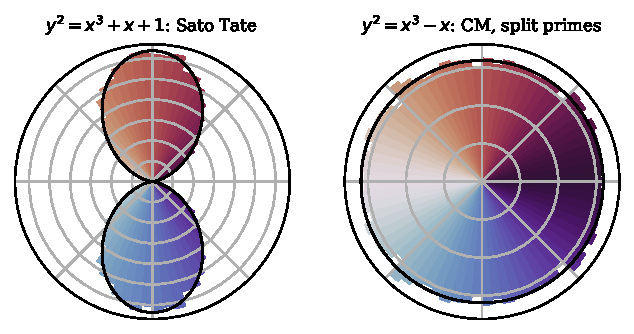
\includegraphics[width=0.92\textwidth]{figs/frobenius_roses.pdf}
\caption{Polar histograms of the Frobenius angles $\pm\theta_p$ for the primes below $4\times10^5$; the radius is the density, the radial labels are omitted, and each panel has its own radial scale. Left: $E_1$, with the Sato Tate density $\sin^2\theta/\pi$ (black). Right: $E_2$, split primes only, with the uniform density $1/(2\pi)$ (black); the inert primes, where $\theta_p = \pi/2$, are omitted.}\label{fig:04roses}
\end{figure}

\section{Complex multiplication and the Weyl fingerprint}\label{sec:04cm}

Suppose now that $E$ has complex multiplication by an order in an imaginary quadratic field $M$. Deuring \cite{deuring1953} showed that $L(s,E) = L(s,\psi)$ for a Hecke Gr\"ossencharacter\index{Hecke Gr\"ossencharacter} $\psi$ of $M$ of infinity type $(1,0)$. For a prime $p \nmid N$ inert in $M$ the curve is supersingular and $a_p = 0$. For $p$ split, $p = \mathfrak p\bar{\mathfrak p}$, we have $a_p = \psi(\mathfrak p) + \overline{\psi(\mathfrak p)}$, and the argument of $\psi(\mathfrak p)/\sqrt p$ is $\pm\theta_p$. Hecke proved \cite{hecke1918} that these angles are equidistributed on the circle. In the language of this chapter, the Weyl criterion on $\mathrm{U}(1)$ applies because the $L$ functions of the unitary characters $(\psi/|\psi|)^n$, $n \ne 0$, are entire and nonvanishing on $\Re s = 1$. By the Chebotarev density theorem half the primes split. Combining these, $(x_p)$ is equidistributed with respect to
\[
\mu_{\mathrm{CM}}(dx) = \frac12\delta_0(dx) + \frac12\,\frac{dx}{\pi\sqrt{4-x^2}}, \qquad x\in[-2,2],
\]
a point mass at $0$ plus an arcsine law. Group theoretically, $\mu_{\mathrm{CM}}$ is the image of Haar measure on the normaliser $N(\mathrm{U}(1))$ of the diagonal torus in $\SU(2)$: the identity component contributes the arcsine law, since a uniform angle $\theta$ gives $2\cos\theta$ arcsine distributed, and the other component consists of elements of trace $0$. The moments are $\int x^{2m}\,d\mu_{\mathrm{CM}} = \frac12\binom{2m}{m}$ for $m \ge 1$.

\begin{proposition}[Weyl fingerprint of the CM law]\label{prop:04cm}
For $n \ge 1$,
\[
\int_{-2}^2 U_n(x/2)\,\mu_{\mathrm{CM}}(dx) = \begin{cases} 1 & 4 \mid n,\\ 0 & \text{otherwise.}\end{cases}
\]
\end{proposition}

\begin{proof}
Under the arcsine law the angle $\theta$ is uniform on $[0,\pi]$, so the continuous part contributes
\[
\frac1\pi\int_0^\pi \frac{\sin((n+1)\theta)}{\sin\theta}\,d\theta = \frac1\pi\int_0^\pi\sum_{j=0}^n e^{i(n-2j)\theta}\,d\theta .
\]
Pairing the terms $j$ and $n-j$ writes the sum as $1$ (present only for $n$ even, from $j = n/2$) plus terms $2\cos((n-2j)\theta)$ with $n - 2j \ne 0$, each of which integrates to $0$ over $[0,\pi]$. So the arcsine average of $U_n(x/2)$ is $1$ for $n$ even and $0$ for $n$ odd. At the atom, $U_n(0) = \sin((n+1)\pi/2) = \cos(n\pi/2)$, which is $0$ for $n$ odd and $(-1)^{n/2}$ for $n$ even. Averaging the two halves gives $0$ for $n$ odd and $\frac12(1 + (-1)^{n/2})$ for $n$ even, which is $1$ when $4\mid n$ and $0$ when $n \equiv 2 \pmod 4$.
\end{proof}

As predicted by the remark after Theorem~\ref{thm:04weyl}, this is the dimension of the $N(\mathrm{U}(1))$ invariants in $\Sym^n$: the torus fixes only the weight zero vector (for $n$ even), and the other component acts on it by $(-1)^{n/2}$.

Figure~\ref{fig:04weyl} shows the fingerprint in our data. For $E_2: y^2 = x^3 - x$ (conductor $32$) and the good primes below $10^7$, the averages at $n = 4, 8, 12$ are $0.9995$, $0.9988$, $0.9979$, and the other averages with $n \le 12$ lie within $0.0018$ of zero. The proportion of these primes with $a_p = 0$ is $0.5002$. The even moments of $x_p$ for $E_2$ are within $0.14\%$ of $\frac12\binom{2m}{m}$ (Table~\ref{tab:05moments}).

\begin{figure}[t]\centering
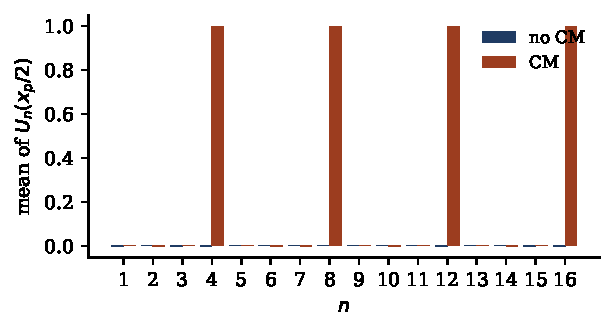
\includegraphics[width=0.8\textwidth]{figs/weyl.pdf}
\caption{Weyl averages $\pi(x)^{-1}\sum_{p\le x}U_n(x_p/2)$ for $1 \le n \le 16$ over the good primes below $10^7$. For $E_1$ (no CM, left bar of each pair) they are close to $0$, the limit that Theorem~\ref{thm:04weyl} requires of a sequence equidistributed for $\ST$; for the CM curve $E_2$ (right bar) they are close to $1$ when $4 \mid n$ and to $0$ otherwise, the limits of Proposition~\ref{prop:04cm}.}\label{fig:04weyl}
\end{figure}

Chapter~\ref{ch:12} turns this separation into a sequential Bayesian test with explicit error exponents.

\section{Joint Sato Tate and coincidences}

For two curves, the pairs $(\theta_p(E), \theta_p(E'))$ are classes in $\SU(2)\times\SU(2)$, whose irreducible representations are $\Sym^m\boxtimes\Sym^n$. By Theorem~\ref{thm:04weyl}, joint equidistribution with respect to $\ST\otimes\ST$ is equivalent to
\[
\frac{1}{\pi(x)}\sum_{p\le x}U_m(x_p/2)\,U_n(x'_p/2) \to 0 \qquad\text{for all } (m,n)\ne(0,0).
\]
By the argument of Theorem~\ref{thm:04serre}, with $(m+1)(n+1)$ in place of $n+1$, this follows if for each $(m,n)\ne(0,0)$ the Rankin Selberg $L$ function $L(s,\Sym^m E\times\Sym^n E')$, with Euler factors
\[
\prod_{i=0}^{m}\prod_{j=0}^{n}\bigl(1-\alpha_p^i\beta_p^{m-i}\alpha_p'^{\,j}\beta_p'^{\,n-j}p^{-s}\bigr)^{-1}
\]
at the primes $p$ of good reduction for both curves (the factors at the finitely many other primes are holomorphic and nonvanishing on $\Re s > 0$, as for a single curve), extends holomorphically to a neighbourhood of $\Re s\ge1$ and has no zeros on $\Re s = 1$. Isogenous curves have equal traces, and a quadratic twist by $\chi$ has $a_p(E') = \chi(p)a_p(E)$, which puts the pairs on the lines $x' = \pm x$; so the right hypothesis is that $E$ and $E'$ are not isogenous over $\bar\Q$.

\begin{theorem}[Joint Sato Tate; Harris \cite{harris2009}]\label{thm:04joint}
Let $E$ and $E'$ be elliptic curves over $\Q$ without complex multiplication that are not isogenous over $\bar\Q$. Then the pairs $(x_p(E), x_p(E'))$ are equidistributed in $[-2,2]^2$ with respect to $\ST\otimes\ST$.
\end{theorem}

Harris \cite{harris2009} reduced the theorem to the potential automorphy of the symmetric powers of $E$ and $E'$ over a common totally real field, and proved it assuming results on the Galois representations attached to automorphic representations of unitary groups that were then expected; those results were established soon afterwards (see the introduction of \cite{blght2011}). Given the automorphy of all symmetric powers \cite{newtonthorne2021,newtonthorne2021b}, the theorem also follows directly from Rankin Selberg theory. For unitary cuspidal automorphic representations $\Pi$ and $\Pi'$, the $L$ function $L(s,\Pi\times\Pi')$ has no zeros on $\Re s = 1$ \cite{shahidi1981}, and it is holomorphic on $\Re s \ge 1$ unless $\Pi' \cong \tilde\Pi\otimes|\det|^{it}$ for some real $t$, in which case its only pole there is a simple pole at $s = 1 - it$ \cite{jpss1983,jacquetshalika1981,moeglinwaldspurger1989}.

For $(m,n)\ne(0,0)$ the hypothesis excludes this exceptional isomorphism when $\Pi$ and $\Pi'$ are the cuspidal automorphic representations attached to $\Sym^m E$ and $\Sym^n E'$, by an argument of Harris that rests on Faltings' isogeny theorem \cite{faltings1983}. Both have trivial central character (symmetric powers of $\SU(2)$ have determinant $1$), while $\tilde\Pi\otimes|\det|^{it}$ has central character $|\cdot|^{it(m+1)}$, so $t = 0$, and the dimensions give $m = n$. Then $\Sym^n\rho_{E,\ell}\cong\Sym^n\rho_{E',\ell}$ for the $\ell$ adic representations on the Tate modules (Chapter~\ref{ch:03}), which, as their images are open in $\GL_2(\Z_\ell)$ (Theorem~\ref{thm:ch3serre}), makes the adjoint representations agree and so forces $\rho_{E',\ell}\cong\rho_{E,\ell}\otimes\eta$ for a character $\eta$, quadratic because both determinants are the cyclotomic character. By Faltings' theorem $E'$ is then isogenous to a quadratic twist of $E$, hence to $E$ over an extension of $\Q$ of degree at most $2$. For curves over $\Q$ without complex multiplication an isogeny over $\bar\Q$ is already defined over such an extension, so our hypothesis is equivalent to Harris's, that $E$ and $E'$ do not become isogenous over an abelian extension of $\Q$.

\begin{corollary}\label{cor:04coinc}
Under the hypotheses of Theorem~\ref{thm:04joint}, the set of primes $p$ with $a_p(E) = a_p(E')$ has natural density zero.
\end{corollary}

\begin{proof}
If $a_p(E) = a_p(E')$ then $x_p = x'_p$, so $(x_p, x'_p)$ lies on the diagonal $\Delta = \{(u,u) : u \in [-2,2]\}$. The set $\Delta$ is closed, and $(\ST\otimes\ST)(\Delta) = \int \ST(\{u\})\,\ST(du) = 0$ because $\ST$ has no atoms. The portmanteau theorem and Theorem~\ref{thm:04joint} give
\[
\limsup_{x\to\infty}\frac{\#\{p\le x: a_p(E) = a_p(E')\}}{\pi(x)} \le (\ST\otimes\ST)(\Delta) = 0. \qedhere
\]
\end{proof}

The heuristic behind the Lang Trotter conjecture (Chapter~\ref{ch:05}) predicts the size of this set. If $a_p(E)$ and $a_p(E')$ were independent integers distributed like $\sqrt p$ times Sato Tate variables, they would agree with probability about $p^{-1/2}\int_{-2}^2 \bigl(\sqrt{4-u^2}/(2\pi)\bigr)^2\,du = \frac{8}{3\pi^2}\,p^{-1/2}$, so the number of coincidences up to $x$ should be of order $\sqrt x/\log x$, with a constant that also reflects congruences between the two curves.

\section{The general Sato Tate conjecture}

By Theorem~\ref{thm:04weyl} and Serre's argument, the general Sato Tate conjecture for an abelian variety $A/\Q$ (Conjecture~\ref{conj:ch3gst}, with $\mathrm{ST}(A)$ as in Definition~\ref{def:ch3stgroup}) follows if the $L$ functions attached to the nontrivial irreducible representations of $\mathrm{ST}(A)$ extend holomorphically to a neighbourhood of $\Re s \ge 1$ without zeros on $\Re s = 1$, a consequence of the Langlands conjectures. For the $52$ groups of abelian surfaces (Theorem~\ref{thm:ch3fkrs}), the moment statistics of the curves that Fit\'e, Kedlaya, Rotger and Sutherland \cite{fkrs2012} exhibit for each group, integer combinations of values of the Weyl fingerprint, match the predicted ones numerically; the conjecture is open for $\mathrm{ST}(A)=\USp(4)$ and known in many other cases, as recorded after that theorem.

\section{Notes}

Weyl's paper \cite{weyl1916} contains the criterion and the equidistribution of polynomial sequences by differencing. The appendix to Chapter I of Serre's book \cite{serre1968} is the standard reference for the compact group version and the source of Theorem~\ref{thm:04serre}. Sato found the $\sin^2$ law numerically; Tate derived it from the expectation that algebraic cycles on powers of $E$ account for the poles of symmetric power zeta functions \cite{tate1965}. Birch \cite{birch1968} proved a vertical version: averaged over all elliptic curves over $\mathbb{F}_p$, the even moments of $a_p/\sqrt p$ tend to the Catalan numbers as $p\to\infty$. Chapter~\ref{ch:06} surveys such vertical laws, and Chapter~\ref{ch:07} treats the one for Hecke eigenvalues.

The route through potential automorphy is surveyed in the introductions of \cite{hsbt2010,blght2011}; the tensor product device of Harris \cite{harris2009} is one of the ingredients of \cite{blght2011}. Newton and Thorne's proof \cite{newtonthorne2021,newtonthorne2021b} combines automorphy lifting with an analytic continuation argument along the Coleman Mazur eigencurve, and Thorner \cite{thorner2021} used their theorem to prove effective forms of Sato Tate. Serre's lecture notes \cite{serre2012} give the general formalism, Sutherland's survey \cite{sutherland2019} describes Sato Tate groups and their moment sequences, and the database \cite{lmfdb} records Sato Tate groups of many curves and abelian surfaces. Katz and Sarnak \cite{katzsarnak1999} develop the analogous theory over finite fields, where Deligne's equidistribution theorem \cite{deligne1980} proves the analogue of the conjecture for families.

Nothing in this chapter proves functoriality: Theorem~\ref{thm:04serre} derives a probabilistic consequence, and the arithmetic input of Theorem~\ref{thm:04STthm} was supplied by others. Proposition~\ref{prop:01limits} records the converse limitation: no statistic of the empirical law of $(x_p)$ alone can detect automorphy.

\section{Exercises}

\begin{enumerate}
\item Show that the irreducible characters of $\mathrm{U}(1)$ are $\theta \mapsto e^{ih\theta}$, $h\in\Z$, and deduce from Theorem~\ref{thm:04weyl}, in the form for sequences indexed by the integers noted after its proof, Weyl's theorem that $(n\alpha \bmod 1)$ is equidistributed for irrational $\alpha$. Show that the same sequence is not equidistributed for any rational $\alpha$ by exhibiting a Weyl average that does not tend to zero.
\item Prove that the arcsine law $dx/(\pi\sqrt{4-x^2})$ on $[-2,2]$ has even moments $\binom{2m}{m}$, by counting all (not only nonnegative) paths of $\pm1$ steps that return to $0$. Deduce the moments of $\mu_{\mathrm{CM}}$, and compare with the Catalan numbers by the ballot theorem.
\item Let $E/\Q$ be an elliptic curve without complex multiplication, and let $g$ be a Riemann integrable function on $[-2,2]$. Show that $\pi(x)^{-1}\sum_{p\le x}g(x_p)$ tends to $\int g\,d\ST$ (approximate $g$ from above and below by continuous functions), and deduce that the primes with $|a_p| \le \sqrt p$ have natural density $\frac13 + \frac{\sqrt3}{2\pi}$.
\item Let $H \subset \SU(2)$ be a finite subgroup and $\mu$ the image on $[-2,2]$, under the trace, of the uniform probability measure on $H$. Show that $\int U_n(x/2)\,\mu(dx)$ is a nonnegative integer for every $n$, and that it is at least $1$ whenever $n$ is a multiple of $2|H|$. Conclude that no such $\mu$ can be the limiting law of $(x_p)$ for a newform without complex multiplication.
\item\label{ex:04clt} (Probabilistic.) Let $Y_1, Y_2, \dots$ be independent with law $\ST$, and $W_n(T) = T^{-1}\sum_{j\le T}U_n(Y_j/2)$. Show that for every finite set $S$ of positive integers the vector $(\sqrt T\,W_n(T))_{n\in S}$ converges in law as $T\to\infty$ to a vector of independent standard normal variables. What changes when the $Y_j$ have law $\mu_{\mathrm{CM}}$? Compute the means and covariances of the $U_n(Y_j/2)$ in that case.
\end{enumerate}

\section{Open computational problems}

\begin{compproblem}[Weyl averages at scale]
Objective: measure how fast the Weyl averages $W_n(x) = \pi(x)^{-1}\sum_{p\le x}U_n(x_p/2)$ tend to zero, and how the rate depends on $n$, for $E_1$ and for the $200$ random curves of Chapter~\ref{ch:05}, for $1 \le n \le 50$ and all primes up to $10^{10}$ (about $4.6\times10^8$ primes per curve). Route: PARI/GP \texttt{ellap} over blocks of primes in parallel, GPU baby step giant step, or Harvey's average polynomial time algorithm \cite{harvey2014}, accumulating $U_n(x_p/2)$ for all $n \le 50$ by the three term recurrence. Deliverable: plots on logarithmic axes of $\sqrt{\pi(x)}\,|W_n(x)|$ against $x$ and $n$, with a fitted law for its growth in $n$. Why it matters: for independent draws from $\ST$ the quantity $\sqrt{\pi(x)}\,W_n(x)$ is asymptotically standard normal for every $n$ (Exercise~\ref{ex:04clt}), while the generalized Riemann hypothesis for $L(s,\Sym^n E)$ gives, through the explicit formula, only $W_n(x) = O(n\,x^{-1/2}\log x\,\log(nNx))$ with $N$ the conductor of $E$ (Chapter 5 of \cite{iwanieckowalski2004}); the data show which of the two describes the dependence on $n$.
\end{compproblem}

\begin{compproblem}[Fingerprints of genus two Jacobians]
Objective: compute the exact Weyl fingerprints of the $52$ Sato Tate groups $G$ of abelian surfaces \cite{fkrs2012}, that is the integers $\int\chi_\rho\,d\mu_G = \dim\rho^G$ for all irreducible representations $\rho$ of $\USp(4)$ with highest weight $(a,b)$, $a \ge b \ge 0$, $a + b \le 12$; find a smallest set of such $\rho$ that separates the $52$ groups, or the pairs that this range cannot separate; and compare the fingerprints with the empirical Weyl averages of the $66{,}158$ genus two curves in the LMFDB (absolute discriminant at most $10^6$), using all primes up to $10^8$. Route: branching from $\USp(4)$ to the identity component of $G$, followed by the action of the component group, in Sage or Magma; $L$ polynomials by the methods of \cite{kedlayasutherland2009} or by the average polynomial time algorithm of \cite{harveysutherland2014}. Deliverable: the table of fingerprints, a minimal separating set of representations, and for each curve the empirical averages on that set with the group they single out. Why it matters: Weyl averages are sufficient in the limit for the Bayesian identification of Chapter~\ref{ch:12}, so a minimal separating set measures how few averages identify a Sato Tate group; agreement for each group that occurs among these curves tests the general Sato Tate conjecture group by group, including groups for which it is not known.
\end{compproblem}

\begin{compproblem}[Joint laws of pairs and twists]
Objective: count the coincidences of Corollary~\ref{cor:04coinc}, and contrast the joint laws of unrelated pairs with those of twists. Problem~3.3 already tests the independence of unrelated pairs, with twists as a control, by joint Weyl averages and discrepancy; here the focus is the density zero set of coincidences. Objects: $10^3$ pairs of curves of conductor below $10^4$ without complex multiplication that are not isogenous over $\bar\Q$, and $E_1$ with its quadratic twists by the fundamental discriminants $d \ne 1$ with $|d| \le 10^3$; all primes up to $10^9$. Route: LMFDB curve lists and PARI/GP \texttt{ellap} in batch; a twist has traces $\chi_d(p)\,a_p(E_1)$ and needs no new point counts. Deliverable: for the unrelated pairs, the counts $\#\{p\le x : a_p(E) = a_p(E')\}$ at $x = 10^6,\dots,10^9$ fitted to $c\sqrt x/\log x$ and compared with $c_0 = 16/(3\pi^2) \approx 0.54$, the value for independent Sato Tate traces, corrected for congruences from the mod $\ell$ images as Lang and Trotter do for $a_p = 0$; and heat maps of the joint Weyl averages $\pi(x)^{-1}\sum_{p\le x}U_m(x_p/2)U_n(x'_p/2)$, $m,n \le 10$, whose limits are $0$ for unrelated pairs when $(m,n)\ne(0,0)$, and for twists $\delta_{mn}$ for even $n$ and $0$ for odd $n$. Why it matters: Corollary~\ref{cor:04coinc} gives only density zero; the constants $c$ are the analogue for pairs of the Lang Trotter constants of Chapter~\ref{ch:05}, and quadratic twists, up to isogeny over $\Q$, are exactly the pairs excluded from Theorem~\ref{thm:04joint}.
\end{compproblem}

